\documentclass[conference]{IEEEtran}
\IEEEoverridecommandlockouts
% The preceding line is only needed to identify funding in the first footnote. If that is unneeded, please comment it out.
\usepackage{cite}
\usepackage{amsmath,amssymb,amsfonts}
\usepackage{algorithmic}
\usepackage{graphicx}
\usepackage{textcomp}
\usepackage{xcolor}
\usepackage{nccmath}
\usepackage{todonotes}
\def\BibTeX{{\rm B\kern-.05em{\sc i\kern-.025em b}\kern-.08em
    T\kern-.1667em\lower.7ex\hbox{E}\kern-.125emX}}
\begin{document}

\title{Growth-Aware Dynamic Reward Scheme For Inflation Optimization In Blockchain Environment \small{V0.1}}

\author{\IEEEauthorblockN{Dr. Tarek Awwad}
\IEEEauthorblockA{\textit{Ki Foundation}\\
tarek@foundation.ki}
\and
\IEEEauthorblockN{Reda Berrehili}
\IEEEauthorblockA{\textit{Ki Foundation}\\
reda@foundation.ki}}

\maketitle

\begin{abstract}
In blockchain environments, the supply inflation policy is a widely adopted approach for compensating block validators for their effort and engagement in securing the network. In the literature, this process consists in creating a fix amount of new token and awarding them to these validators. This, naturally, increases the token supply and thus can have a negative impact on the token value if the created inflation is not coupled with an increasing usage of the network and its token. In this document we present a novel reward scheme that consists in dynamically adapting the block reward to the network usage in order to optimize the yearly inflation while maintaining the fairness and attractiveness of the network.
\end{abstract}

\section{Introduction}
As a Distributed Ledger Technology, the blockchain paradigm consists in replacing the central trusted authorities (e.g., banks) that perform the task of maintaining, validating and synchronizing assets and transaction data in traditional centralized systems, by a set of interconnected peers. These peers invest knowledge, work time and computational power in order to secure the network and maintain the integrity of the blockchain through the block validation process, which in turn is ruled by a consensus protocol. To compensate these peers for their engagement, they are awarded a given amount of tokens - which represents the value unit in the system - for each validated block. The reward tokens are, usually, not part of the initial token supply. Instead they are created at each block validation which increases this supply. In practice, this is known as the inflation process. Many existing blockchain systems uses this supply inflation process to incentivize their validators. For instance, in Ark, Ethereum and Lisk blockchains, 2 ARKs, 2 ETHs and 3 LSKs are created and awarded at each block validation respectively. In 2018, this was equivalent to arround 5\%, 4.7\% (down from 7.3\%) and 4\% of yearly inflation (i.e., percentage of created tokens in the total token supply) resp.
%https://github.com/ethereum/EIPs/blob/master/EIPS/eip-1234.md
%https://steemit.com/ethereum/@zeroshiki/inflation-comparison-lisk-vs-ethereum

In classical economical systems, an inflation that is not accompanied with a fair velocity of the money (i.e., people spending more), decreases the facial value of this money. The same applies in blockchain systems where an increasing usage of the system and its token is necessary to absorb the negative impact of "printing money". This is particularly true at the launch of a network where the usage of the token, measured by the number of transactions, is low. Therefore, adapting the inflation rate to the actual activity on the network is crucial for maintaining the value of the incentive token. This, however, should not be  achieved at the cost of the validators' incentive of participating in the early stages of the blockchain life.

To address this challenge, the Ki Foundation proposes a dynamic reward computation scheme that takes into account the number of transactions being made on the blockchain to optimize the yearly inflation rate. The proposed scheme ensures that the validators are incentivized to join since the early stages by guaranteeing a fixed base payment adjusted on an milestone basis.

This paper is organized as follows :  in Section \ref{sec:discussion}, the intuition and vision behind the proposed approach are discussed. Then, the reward computation scheme is described in details in Section \ref{sec:scheme}. Finally, experiments on real and simulated data are given in Section \ref{sec:experiements} before concluding this document in Section \ref{sec:conclusion}.

\section{Preliminary discussion}
\label{sec:discussion}
Like the vast majority of existing blockchains, the Ki blockchain rewards validators through the inflation of supply. Tokens are minted on the creation of every new block and awarded to the block validator. As explained earlier, to secure the value of the token, there needs to be tight link between the number of created tokens and the actual usage of the tokens (i.e., the token velocity in the system) and the network. This usage - of both the network and the token - can be expressed in terms of the number of transactions achieved on the blockchain. A low number of transactions reflects a low network usage and a low token velocity \footnote{assuming that the tokens are not concentrated in a limited number of wallets}. Hence, we leverage here the number of transactions per block as an indicator of the network and token usage to optimize the  supply inflation process.

An extreme mechanism that could be used to achieve this value-centric control, is to award a block validator an amount of tokens proportional to the number of transaction found in the block they have validated. This means, that the reward will be slashed for empty blocks and will be extremely low for blocks with very few transacitons. Whilst this allows to avoid the “bad” inflation, a zero reward for an empty block can negatively impact the validators and their incentives, particularly during the early stages of the network, when empty blocks constitute the vast majority of the validated blocks. That is because validators will be investing with a zero Return On Investment (ROI). Therefore, a validator should be guaranteed a base payout regardless the payload of the created block. Consequently, the reward function must involve both a static and a dynamic reward factor. The first ensures the base payout (at least during critical periods), and the second ensures that the number of created tokens is controlled and adjusted in relation to the intended yearly inflation rate. In order to minimize the negative impact of the fixed reward paid for empty blocks, its amount can be optimized by adapting it according to the ratio of empty blocks over the validated ones. That is, the fixed reward should be adjusted over a period of time. For instance, this can be done on a yearly basis through tuning the static split of the inflation rate. Eventually this reward will tend to its minimal value.

In practice, the dynamic part of the reward can be computed in two ways. On one hand, it can be computed on a block basis. That is, the yearly created tokens can be distributed over the number of blocks to be validated for the year. Since the number of validated blocks per year is an intrinsic parameter of the blockchain, this computation is deterministic. However, the limitation of the block based computation is its coarse granularity. That is, it occurs yearly and is independent from the number of transactions circulating on the network. This is not inline with our initial assumption stating that the number of transactions is indeed the real indicator of the usage of the network and thus how viable it is. On the other hand, the dynamic part of the reward can be computed with regards to the number of transactions per year. That is, the reward paid per block is equal to the total rewards paid for the individual transactions contained in the block. In this case, the yearly created tokens are distributed over the number of transactions performed during the year. This allows for a more fine grained reward computation. The drawback here, is that the number of transactions is not a configurable parameter of the blockchain, thus not deterministic. In other words, the dynamic reward here relies on not only a yearly growth projection, but also the trend of this growth. Hence, a forecasting function is needed.

In summary, we propose a reward computation function with 2 components. A static component adjusted yearly and a dynamic component proportional to the number of transaction per block and adjusted with respect to the growth projection and trend of the network in terms of transaction number.

\section{The Dynamic Reward function}
\label{sec:scheme}
In this section, and based on the previous discussion, we describe  a novel dynamic reward scheme that ensures a tight relation between the network usage and the yearly inflation while guaranteeing a real incentive for the validators to join the blockchain as early as its launch.

\subsection{Setup}
\label{setup}
We start by defining the global constants of the environment. Let  $I$ be the number of created tokens for the year i.e. the inflation. Let $B$ be the number of validated blocks for the year. And let $T_{max}$ be the maximum number transactions that can be found in a block $b$.

Second we define the variables of the system. Let $t$ denote a transaction, $R_b$ denote the reward paid for a block $b$ and $T_b$ denote the transactions found in $b$. $\hat{T}$ denotes the estimated number of transactions for the year, $\bar{T}_b$ denotes the remaining transactions for the year after block $b$ and $\bar{B}_b$ denotes the remaining blocks for the year after block $b$.


From the aforementioned constant and variables we derive the variables specific to our approach. Let $f_b$ denotes the filling rate of a block. It can be expressed as shown in Equation~\ref{eq:filling}.

\begin{equation}
        f_b=\frac{T_b}{T_{max}}
        \label{eq:filling}
\end{equation}

Finally let $sI$ be the static inflation and $dI$ be the static inflation. That is :
\begin{equation}
    I=sI+dI
    \label{eq:inflationsplit}
\end{equation}


\subsection{Reward computation}
The total reward to be paid per validated block is equal to the sum of two elements. A static element (sR) and a dynamic element (dR). That is :

\begin{equation}
		R_b = sR_b +dR_b
\end{equation}

Since the total amount of paid reward is fixed by the inflation for the current year, one has:

\begin{equation}
		\sum_{b=1}^{B}R_b=\sum_{b=1}^{B}(sR_b +dR_b) =sI + dI = I
\end{equation}

As mentioned above, the static part of the reward serves as an incentive for the validators by guaranteeing them a minimal payout based on their validation effort. Therefore, the validators  need to be paid for each block validated, regardless of its payload and the moment at which it is validated. Accordingly, the static reward (sRb) given to a validator for validating a block is equal to:

\begin{equation}
		sR_b=\frac{sI}{B}
\end{equation}

On the other hand, the second part of the reward i.e. the dynamic reward ($dR_b$) adjusts the total reward according to the evolution of the network (from a transaction point of view) and guarantees the balance between a fair reward scheme and a controllable token creation. Indeed, if we assume that the total amount of created tokens for a given year is fixed and predefined at the beginning of the year, then, at a given instant ($t$), the amount of tokens that can be created and rewarded to the validator is equal to the remaining quota of created tokens for the year divided by the number of remaining blocks to be validated for the year. This is equivalent to distributing the dynamic reward over the blocks to be created during the year. Firstly, this renders the dynamic reward static and, secondly, does not take into account the evolution of the network from a transaction perspective. To tackle this problem, we propose the following: first a theoretical dynamic Reward (tdR) is computed by distributing the dynamic inflation over the number of blocks. That is:

\begin{equation}
			tdR_b=\frac{dI}{B}
\end{equation}

Then, each block b is paid a fraction of $dR_b$ computed proportionally to the filling rate $f_b$ (see Section "Setup'') of this block. That is:

\begin{ceqn}
	\begin{align}
		dR_b=f_b \times tdR_b
	\end{align}
\end{ceqn}

Indeed, unless the filling rate is equal to 1 (that is when the block is full), a part of the theoretical reward, which we denote $\bar{dR}_b$, is not spent. It can be expressed as follows:
\begin{ceqn}
	\begin{align}
		\bar{dR}_b=td_R - tdR_b
	\end{align}
\end{ceqn}

Here, one can act in two different manners: (i) $\bar{dR}_b$ is dropped from the inflation computation or (ii) $\bar{dR}_b$ is redistributed. In the next paragraphs these two strategies are explained and discussed.

Suppose that $\bar{dR}_b$ is left over and only the tokens needed to reward the block with regards to its filling rate (Eq. 5) are created. On the one hand, this allows us to minimize the inflation by only paying the actual transactions. On the other hand, this might be non-incentivizing to the validators in the early phases of the blockchain's life. Indeed, the block filling rates are very low during these periods, which means that dynamic rewards might be extremely low.

Suppose that $\bar{dR}_b$ is created (partially or entirely) and redistributed over the remaining blocks. By redistributing the remaining part of $tR_b$, one adjusts the dynamic reward with regards to the actual usage of the network, consequently solving the low filling rate problem. The counterpart of this strategy is that the resulting inflation is less faithful to the actual usage of the network. While not optimal, this still a better choice for network vitality as it retains the validators' interest. Therefore, we adopt this strategy and formalize it as follows. The amount of Ki awarded to a validator for validating a block is equal to:

\begin{ceqn}
	\begin{align}
		dR_b=f_b  \times ( tdR_b + \frac{I}{B-b} \sum_{j=0}^{b} \alpha \times \bar{dR}_j)
	\end{align}
\end{ceqn}

This formula can be expressed in the following words. At each block, the payable amount for a full block is increased by distributing the transferred reward from the previous unfilled blocks over the remaining block to be validated during the year. The paid amount is proportional to the filling rate of the block. Note that $\alpha$ is a hyper-parameter that determines the transferable portion of the unpaid reward. While adapting the reward to the actual transaction load on the network, the strategy explained above might result in the accumulation of the dynamic reward on the final blocks of the year. In other words, validating a block at the end of the year will, unjustifiably, be awarded with a large number of tokens. This is not ideal. Practically, this might be caused by the low filling rate at the network launch, which translates into a large amount of transferred rewards. To counterbalance this, we propose to use the real filling rate, which we denote $f_b$, instead of the theoretical filling rate. $f_b$ is continuously updated every $x$ blocks by using the last x blocks to forecast the load for the upcoming x blocks. The following parameters need to be determined:

\begin{itemize}
	\item The update frequency determined by $x$.
	\item The forecasting function.
\end{itemize}

In the experimental section we study the impact of different forecasting function on the evolution of the block reward over the year and on the achievable gain on the goal inflation rate.

\subsection{Static reward yearly adaptation}
Awarding block validators accordingly with the filling rate and transferring the reward leftovers to remaining blocks, ensure a growth-aware inflation and a validator advantageous reward respectively. Indeed, if the dynamic inflation rate is too small the degree of freedom that one have in adapting the reward is limited. For a fixed yearly inflation rate, a high static split implies a low dynamic split. The former is not justified unless a high incentive for the validators is needed to bootstrap the network. To take this into account, we split the blockchain life into epochs, each of which is defined by the ratio of empty blocks validated on the network. To each epoch a parameter $\rho \in [0, 1]$ is associated. This parameter determines the portion of the inflation ($I$) to be paid as static reward ($sI$). Accordingly, Equation \ref{eq:inflationsplit} can be rewritten as follows:

\begin{equation}
    I=\rho \times sI + (1 - \rho) \times dI
    \label{eq:inflationsplitRho}
\end{equation}

The values of $\rho$ are determined at the launch of the blockchain. When the network starts, empty blocks constitute the vast majority of the validated blocks, validators must be incentivized to participate, thus a larger split of the goal inflation should be paid statically. The less frequent empty blocks are, the smaller the static inflation is.

\section{Experimental study}
\label{sec:experiements}
In this section the experimental study showing the relevance of our approach is described. The study is three folds. First we study the impact of the forecasting function on the achieved inflation rate. Second, the benefit of updating the static split for each epoch is shown. Finally, The impact of this dynamic reward on the ROI on the individual validators is measured.

\begin{table*}[t]
	\centering
    \def\arraystretch{2}
	\caption{The comparison forecasting functions.}
	\begin{tabular}{|l|l|}
		\hline
		Method & Description \\
		\hline\hline
		Theoretical Max & The maximum number of tx per block fixed by the network\\
		\hline
		Prac. Max, Mean & The average number of tx per block over the reference period  \\
		\hline
		Prac. Max, 2 x Mean & Twice the average number of tx per block over the reference period \\
		\hline
		Prac. Max, Max & The maximum number of tx per block over the reference period \\
		\hline
		Prac. Max, 2 x Max & Twice the maximum number of tx per block over the reference period \\
		\hline
	\end{tabular}
\label{tab:forecast}
\end{table*}

\textbf{Experimental setup -} We considered the Bitcoin network as a real life source of data to simulate a realistic evolution of the transaction number and transaction distribution over the validated blocks over a  10 year period ([2009-2018]).

\subsection{The forecasting function impact}
To demonstrate the impact of the forecasting function on the computation of the reward function, we run an experimental study detailed hereafter. We set the yearly inflation rate to 5\% and the static reward split to 20\% of the total inflation. That is equivalent to 1\% of the total supply. For the sake of clarity, we \emph{separately} computed the total inflation rate achieved for each year using 6 naive forecasting models. These are shown in Table \ref{tab:forecast}. The reference period, i.e. the number of historical blocks used to predict the practical maximum number of transactions for the upcoming period were fixed to 144. This is equivalent to one day. Consequently, the frequency of updating the practical maximum is once a day.

Figure~\ref{fig:sim} shows the results of the experiments. The transaction growth (Avg. Yearly. Tx) over the 10 year period is also shown for reference. It is clear that the best way of following the actual transaction growth is to use the theoretical average. That is because the latter directly transcribes the actual usage of the network with regards to its theoretical capacity. However, the problem here is that when bootstrapping the system, the blocks are almost empty. Hence, the filling rate is very low. This means that only the static reward would be paid. This is what occurs for the first year (2009) where the total paid reward is almost equal to 1\% i.e. the mere static reward. This can be discouraging for the validators especially if the theoretical maximum transactions per block is set to high values for scalability concerns.

As explained earlier in Section \ref{sec:scheme}, the practical maximum can solve this limitation. One can approximate this practical maximum by looking to the previous day transactions and assuming that the average or the maximum of the previous day approximate the average and maximum for the current day. The green and red curves show how these basic predictors behave. Clearly, when the growth is subtle (i.e., from 2009 to 2012), these predictors succeed in reflecting this growth and adapt the inflation rate accordingly. However, when the growth becomes more accentuated (i.e. starting 2012), one can see that the set maximum inflation rate is consistently reached. That is because, when the network grows dramatically, the maximum or the average function produces practical maximum values that are way lower than the reality causing the filling rate to reach one and the complete reward to be paid regardless the actual payload of the blocks. Amplifying these functions by a certain factor (e.g., a factor of 2 in this experiment) helps solve this problem as shown by the orange curve. Yet, this is a data dependent result and a more generic predictor needs to be used.

\begin{figure}[h]
	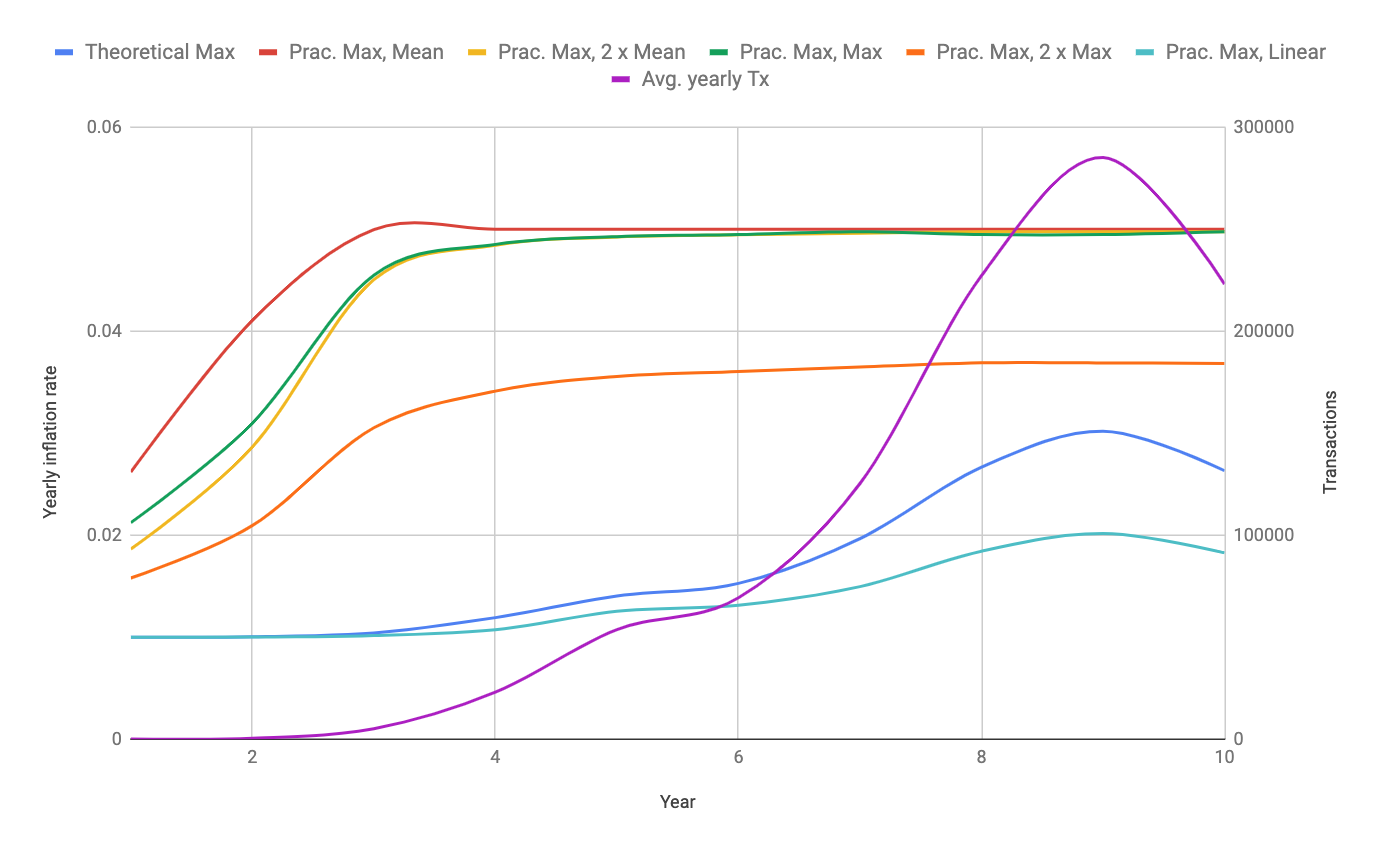
\includegraphics[width=\linewidth, trim= 0cm 1cm 0cm 1cm, clip]{Figures/expU.png}
	\caption{The inflation growth over 10 years with regards to different forecasting methods. (Inflation computed w.r.t. the initial supply. Objective inflation and static inflation unchanged over years)}
	\label{fig:sim}
\end{figure}

\begin{figure}[]
	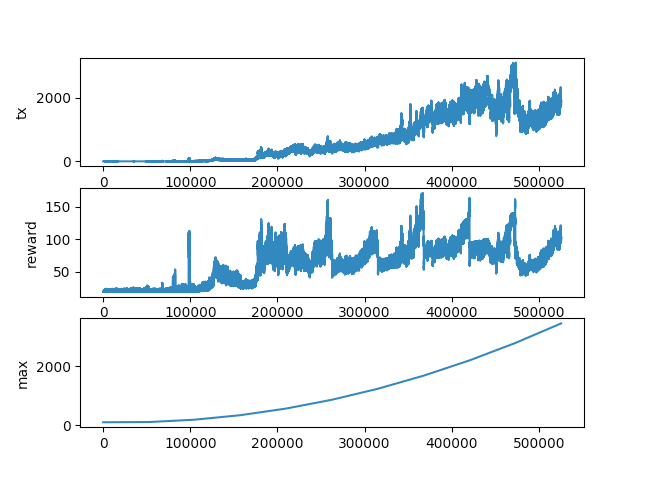
\includegraphics[width=\linewidth, trim= 0cm 0cm 0cm 0cm, clip]{Figures/Figure_continuous.png}
	\caption{The inflation growth over 10 years for a linear yearly forecasting function. (slope adjusted every year)}
	\label{fig:sim}
\end{figure}

It is clear, according to the random walk theory, that it is impossible to accurately predict the evolution of the transaction numbers, and hence of the practical maximum. Nonetheless, our goal is not to perform an accurate estimation but a rough upper bound estimation that allows a fair realistic reward and resiliency to the sudden evolution that can be caused by market factors or intended attack (e.g. maxing out the blocks payload). Tuning both the update frequency and the forecasting function are needed to accomplish this goal.

\begin{figure*}[]
	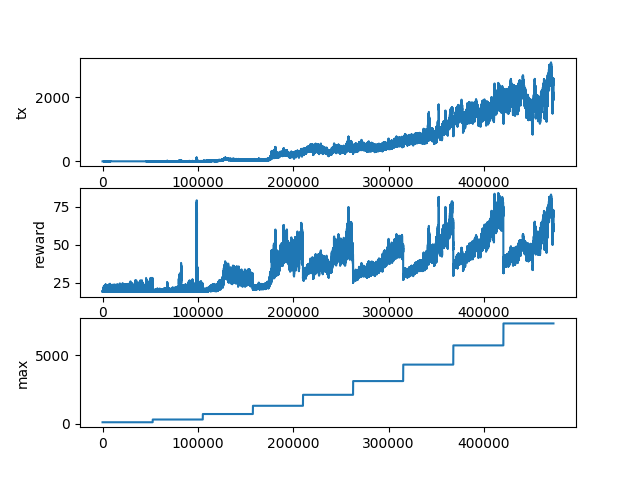
\includegraphics[width=0.49\linewidth, trim= 0cm 0cm 0cm 0cm, clip]{Figures/Figure_steps.png}
	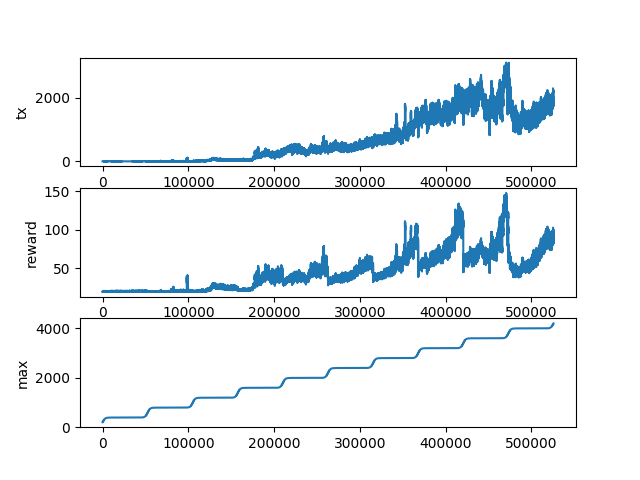
\includegraphics[width=0.49\linewidth, trim= 0cm 0cm 0cm 0cm, clip]{Figures/Figure_steps_smooth.png}
	\caption{The inflation growth over 10 years for a step forecasting function. (Right: with a smoothing factor, Left: without a smoothing factor)}
	\label{fig:sim}
\end{figure*}

\section{Discussion}
In our model, the amount of the reward paid per block is proportional to the filling rate of this block. Indeed, this might incentivize some validators to fill up their block to get the highest possible payment. A validator can achive this by preparing the transactions and not broadcasting them until they are the next block producer. As a result, the dynamic reward computation will be altered. Nevertheless, our approach does not aim at minimizing an unbound inflation rate. Instead, it aims at spending as little as possible of a preset bound inflation rate. If every validator started filling up their blocks, the worst that could happen is that all of the preset inflation rate is spent. This is what happens in traditional blockchains. In spite of this, a couple of the method's characteristics help prevent similar misbehaviour. They are detailed in the next paragraphs.

\paragraph{The forecasting function} The more transactions circulate on the network, the higher the upper bound of the block payload predicted by the forecaster is. It is more likely (if a forecasting function is well chosen) that the growth of this upper bound will be exponential over the years (rather then linear). Consequently, if every one wants to fill up their blocks during the whole year, they will need to launch more and more transactions to a point where transaction fees become very high (the theoretical max being very high).

\paragraph{The transaction volume} This is an element that we aim at adding to the reward computation to complement the number of transactions. It would help prevent the ``filling your own block'' attack vector. A validator, who is willing to fill up their blocks, will need to have enough wallets\footnote{If he has only one or very few wallets the reputation system can easily detect a malicious behaviour.} with enough funds and to juggle with his funds all the time to achieve a high transaction volume in their blocks and thus a high rewards.

\paragraph{The reputation system} In addition to the aforementioned discussion, a precision about the context in which the dynamic reward is implemented is due. The Ki blockchain uses a consensus protocol called ``Proof of Reputation'' (PoR). PoR can be briefly explained as follows: actors on the blockchain are characterized by a set of anonymous features related to their behavior, staking and community trustworthiness. These allow to compute a reputation metric for them. Validators with high reputation scores are eligible for block validation slots. Computing this reputation also enables a reputation based accountability. When a validator is trying to fill up their blocks, a high  (Validated a filled block) / (validated a block) ratio can be remarked over time indicating a malicious behaviour. Consequently, the behavioural reputation score of this validator is penalized and they might no more be selected to validate blocks.


\section{Conclusion}
In this document, we described the block validation rewarding approach within the Ki blockchain. It consists of an epoch-based static part paid for each block regardless its payload. To this a dynamically computed part is added. The latter is proportional to the filling rate of the block in terms of the number of transaction and a forecast prediction of the maximal payload of the block. This scheme helps conserve the value of the token by tightening the inflation to the real usage and growth of the network. Moreover, it ensures a fair incentive for the validators to join since the early stages of the network life. One idea that we would like to study in the fututre is to measure the activity of the network not only by the number of transactions but also their volume. Moreover, while we aim in this document at a 5\% of maximum yearly inflation, it is crucial to define governance rules that allow to adapt this maximum inflation rate to the actual value of the token. This adaption is to be performed on an epoch basis, where epoch are defined by the value of the token and the incentives that need to be provided to the system actors to ensure the growth of the network.

\label{sec:conclusion}
\end{document}
